\chapter{Advanced Tie Points}

%=======================================================================================================
\section{Changing default detector in {\tt  XML\_User/}}


There exist different implemantation of Sift detector and Ann matchor in MicMac. The newest one offer
more option, while the oldest have been more tested \dots 

To change the default behaviour you must edit your {\tt MM-Environment.xml} in the folder {\tt include/XML\_User/}.
For example :



\begin{verbatim}
<MMUserEnvironment>
    <TiePDetect> mm3d:Digeo </TiePDetect>
    <TiePMatch > mm3d:Ann </TiePMatch>
</MMUserEnvironment>
\end{verbatim}

Note that the {\tt mm3d:Digeo} implementation of SIFT detector offers several advantages :

\begin{enumerate}
   \item faster, specially in the gaussian computation;

   \item you can use the {\tt NoMax} and {\tt NoMin} options in {\tt Tapioca}, to supress the Min (or Max) in sift detection.
         This divides by $2$ the number of tie points, while conserving the same
         multiple tie point ratio (as at $99.99\dots \%$ a max is never a good homolog of a min).
\end{enumerate}

The default tie point detector is {\tt mm3d:Sift}.


%=======================================================================================================
\section{Filtering tie points in {\tt HomolFilterMasq}}


This command can be used when you have the necessary spatial information to retrieve false
tie points.

The command {\tt HomolFilterMasq} can do some filtering on tie points. The masking
process can be purerly in image geometry or can be done in some ground geometry.

\begin{verbatim}
 mm3d HomolFilterMasq
*****************************
*  Help for Elise Arg main  *
*****************************
Mandatory unnamed args : 
  * string :: {Full name (Dir+Pat)}
Named args : 
  * [Name=PostPlan] string :: {Post to plan, Def : toto ->toto_Masq.tif like with SaisieMasq}
  * [Name=GlobalMasq] string :: {Global Masq to add to all image}
  * [Name=KeyCalculMasq] string :: {For tuning masq per image}
  * [Name=KeyEquivNoMasq] string :: {When given if KENM(i1)==KENM(i2), don't masq}
  * [Name=Resol] REAL :: {Sub Resolution for masq storing, Def=10}
  * [Name=ANM] bool :: {Accept no mask, def = true if MasqGlob and false else}
  * [Name=ExpTxt] bool :: {Ascii format for in and out, def=false}
  * [Name=PostIn] string :: {Post for Input dir Hom, Def=}
  * [Name=PostOut] string :: {Post for Output dir Hom, Def=MasqFiltered}
  * [Name=OriMasq3D] string :: {Orientation for Masq 3D}
  * [Name=Masq3D] string :: {File of Masq3D, Def=AperiCloud_${OriMasq3D}.ply}
  * [Name=SelecTer] Pt2dr :: {[Per,Prop] Period of tiling on ground selection, Prop=proporion of selected}
\end{verbatim}

The main option are :

\begin{enumerate}
    \item {\tt PostPlan} for example set {\tt PostPlan=titi} if there is masq per image and for each image 
          {\tt Image.tif} the masq if {\tt Image\_Masqtiti.tif}, by default will generate an error if this
          image does not exist, set {\tt ANM=true} if you know that non existing images are normal;

    \item {\tt GlobalMasq} if masq common to all images exist (for example with fiducial marqs);

    \item {\tt KeyCalculMasq} , sometime you may have many images and a few masq, each masq being applyable
          for a group of images; use this option with much be a computation key desrcibed in
          {\tt MicMac-LocalChantierDescripteur.xml}

    \item {\tt Masq3D} , a file for 3D masq as seized by {\tt SaisieMasqQT}, the orientation {\tt OriMasq3D} 
          must be initialized;

    \item {\tt SelecTer} , can be used to decrease the number of tie points while maintaining the proportion
          of multiplicity;  if {\tt SelecTer=[Per,Prop]}, then in each tile of size $S=Per*Resol$  in the ground coordinate
          \footnote{$Resol$ being the average ground resolution} the point are selected in the subtile of 
          size $S * \sqrt{Prop}$
    
    
\end{enumerate}



%=======================================================================================================

\section{Merging Tie point from multiple view with {\tt HomolMergePDVUnik}}

This command correspond to rather special case, when you have a set of camera that do not move (or form a rigid block) and the scene is moving.
For example :

\begin{itemize}
    \item there is three fixed camera $A,B,C$;
    \item at time $1,2,3,4$ someone is moving in fornt of the camera and the images $A_1,A_2, \dots C_3,C_4$ were acquired ;
\end{itemize}

It is not possible to make some standard photogrammetric processing on $A_1,A_2, \dots C_3,C_4$ as the scene is not static.
By the way if we knew the pose  $P_A,P_B,P_C$ of the camera, then  all the homologous points $(A_1,B_1), (A_2,B_2) \dots (A_4,B_4)$ 
would be compatible witj $P_A$ and $P_B$, which means that we can merge this tie points in a unique file that can be used
to estimate $P_A$ and $P_B$; and the same with $A,C$ and $B,C$. 


The command  {\tt HomolMergePDVUnik} does this merging, in fact you can consider that the tie-points 
obtained are more or less resulting are some kind of merging from the different scene. 

\begin{verbatim}
mm3d HomolMergePDVUnik
*****************************
*  Help for Elise Arg main  *
*****************************
Mandatory unnamed args : 
  * string :: {Full name (Dir+Pat)}
  * string :: {Dir of external point}
Named args : 
  * [Name=PostIn] string :: {Post for Input dir Hom, Def=}
  * [Name=PostOut] string :: {Post for Output dir Hom, Def=MasqFusion}
  * [Name=ExpTxt] bool :: {Ascii format for in and out, def=false}
  * [Name=DirN] vector<std::string> :: {Supplementary dirs 2 merge}
\end{verbatim}



%=======================================================================================================
\section{Tie points on low contrast images usign {\tt SFS} in {\tt MicMac-LocalChantierDescripteur.xml}}


The current implementation of SIFT++ used in MicMac is not fully invariant to scaling/translation in radiometry. This may be a problem in case of acquisitions having a good SNR but with low contrast in the scene; in this case, thanks to good SNR there is potential information to get tie points, but as this information is assimilated to noise, it cannnot be extracted.

To overcome this problem, it is possible to require that MicMac computes some contrast enhancement on images before computing SIFT points. Although this method is not optimal (it would be better to modify the SIFT++ Kernel), it has the advantage of existing\dots



The figure~\ref{FIG:SF:Det} presents an image without enhancement, in its original form, and the same image after enhancement. The figure~\ref{FIG:SF:TieP} presents the detected tie points; we notice that the spatial density of tie points is much higher on enhanced image.

Of course, the enhanced images are fairly artificial, as it can be seen on figure~\ref{FIG:SF:Img} that presents a full image before and after enhancement. So if this option is activated, the enhanced images are used only for the tie points steps (which are developed as specific "hidden files" in folder {\tt Tmp-MM-Dir}).


To activate this option, the {\tt NKS-Assoc-SFS} must be changed in the {\tt MicMac-LocalChantierDescripteur.xml}. It must return {\tt SFS} instead of the default value {\tt NONE}. For example:

\begin{verbatim}
    <KeyedNamesAssociations>
        <Calcs>
            <Arrite>  1 1 </Arrite>
            <Direct>
                <PatternTransform> .* </PatternTransform>
                <CalcName>  SFS </CalcName>
            </Direct>
        </Calcs>
        <Key>   NKS-Assoc-SFS </Key>
    </KeyedNamesAssociations>
\end{verbatim}

\begin{figure}
\begin{center}
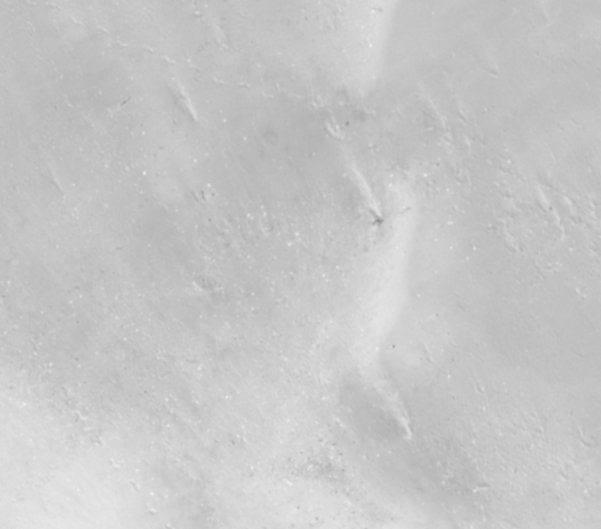
\includegraphics[width=0.4\textwidth]{FIGS/Tapioca-SFS/Detail-STD.jpg}
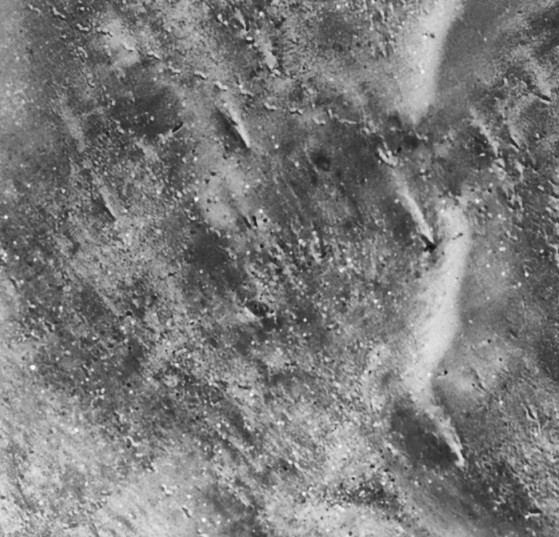
\includegraphics[width=0.4\textwidth]{FIGS/Tapioca-SFS/Detail-SFS.jpg}
\end{center}
\caption{Detail of image before and after enhancement}
\label{FIG:SF:Det}
\end{figure}


\begin{figure}
\begin{center}
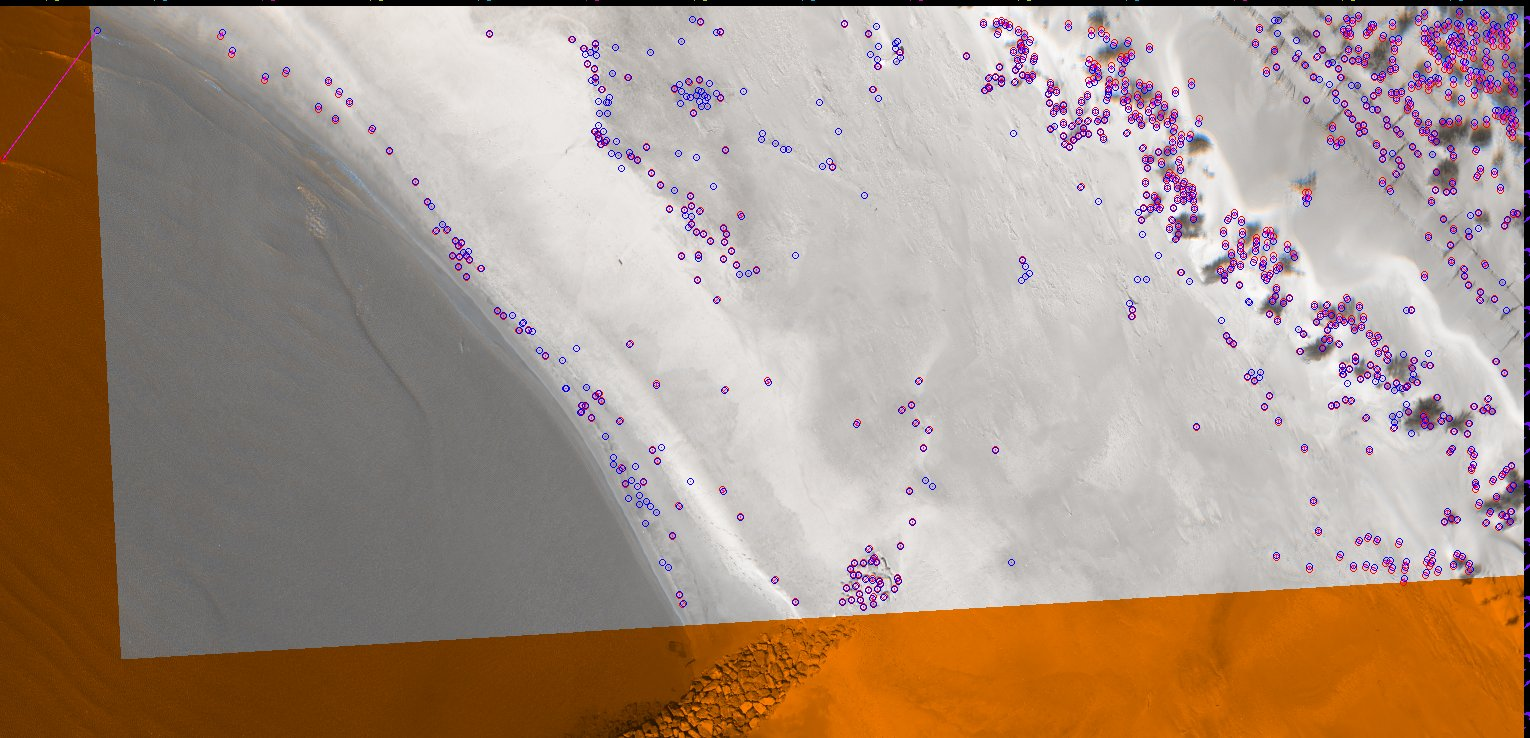
\includegraphics[width=0.95\textwidth]{FIGS/Tapioca-SFS/SIFT-STD.jpg}
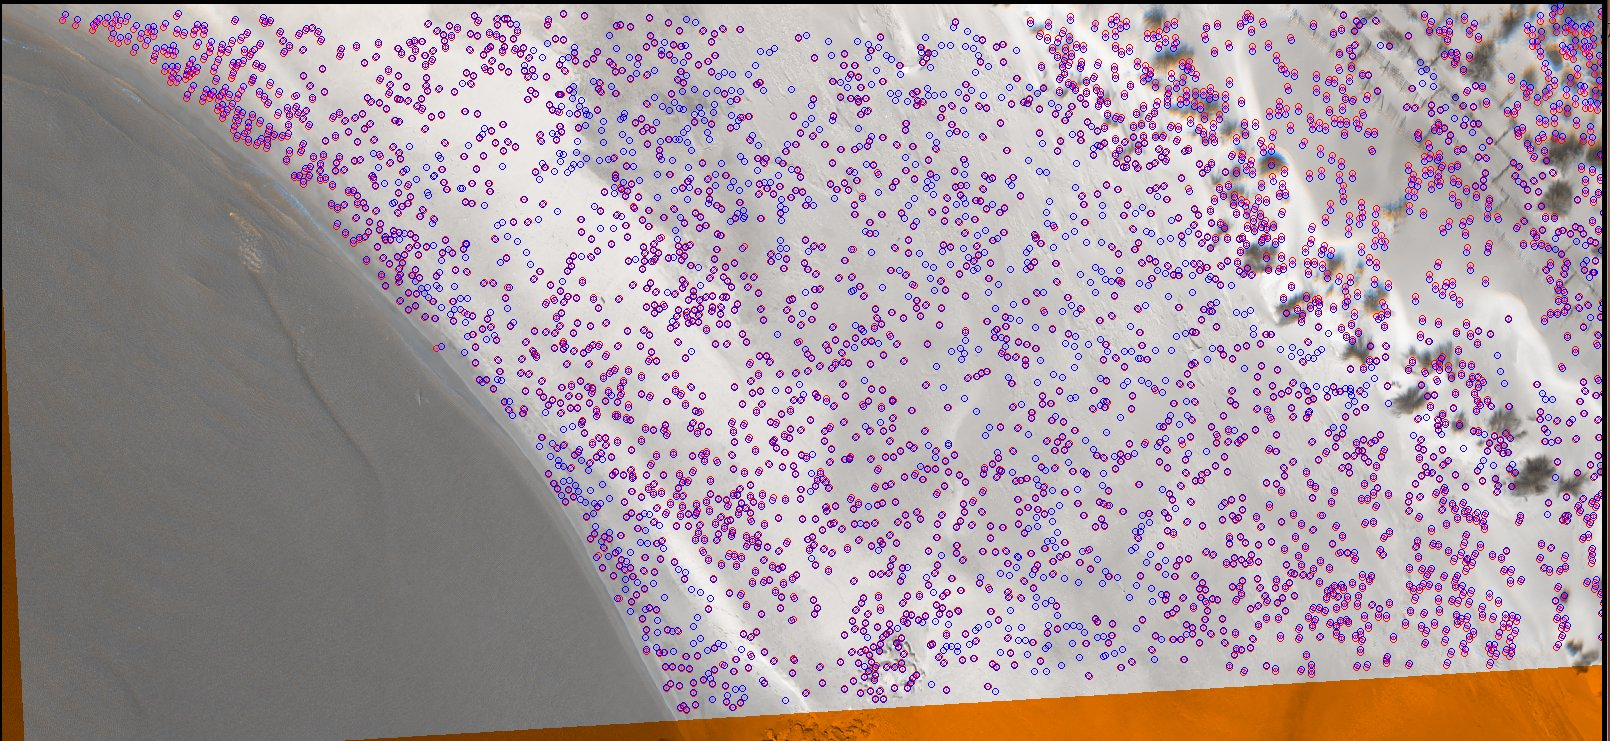
\includegraphics[width=0.95\textwidth]{FIGS/Tapioca-SFS/SIFT-SFS.jpg}
\end{center}
\caption{Tie points before and after enhancement}
\label{FIG:SF:TieP}
\end{figure}

\begin{figure}
\begin{center}
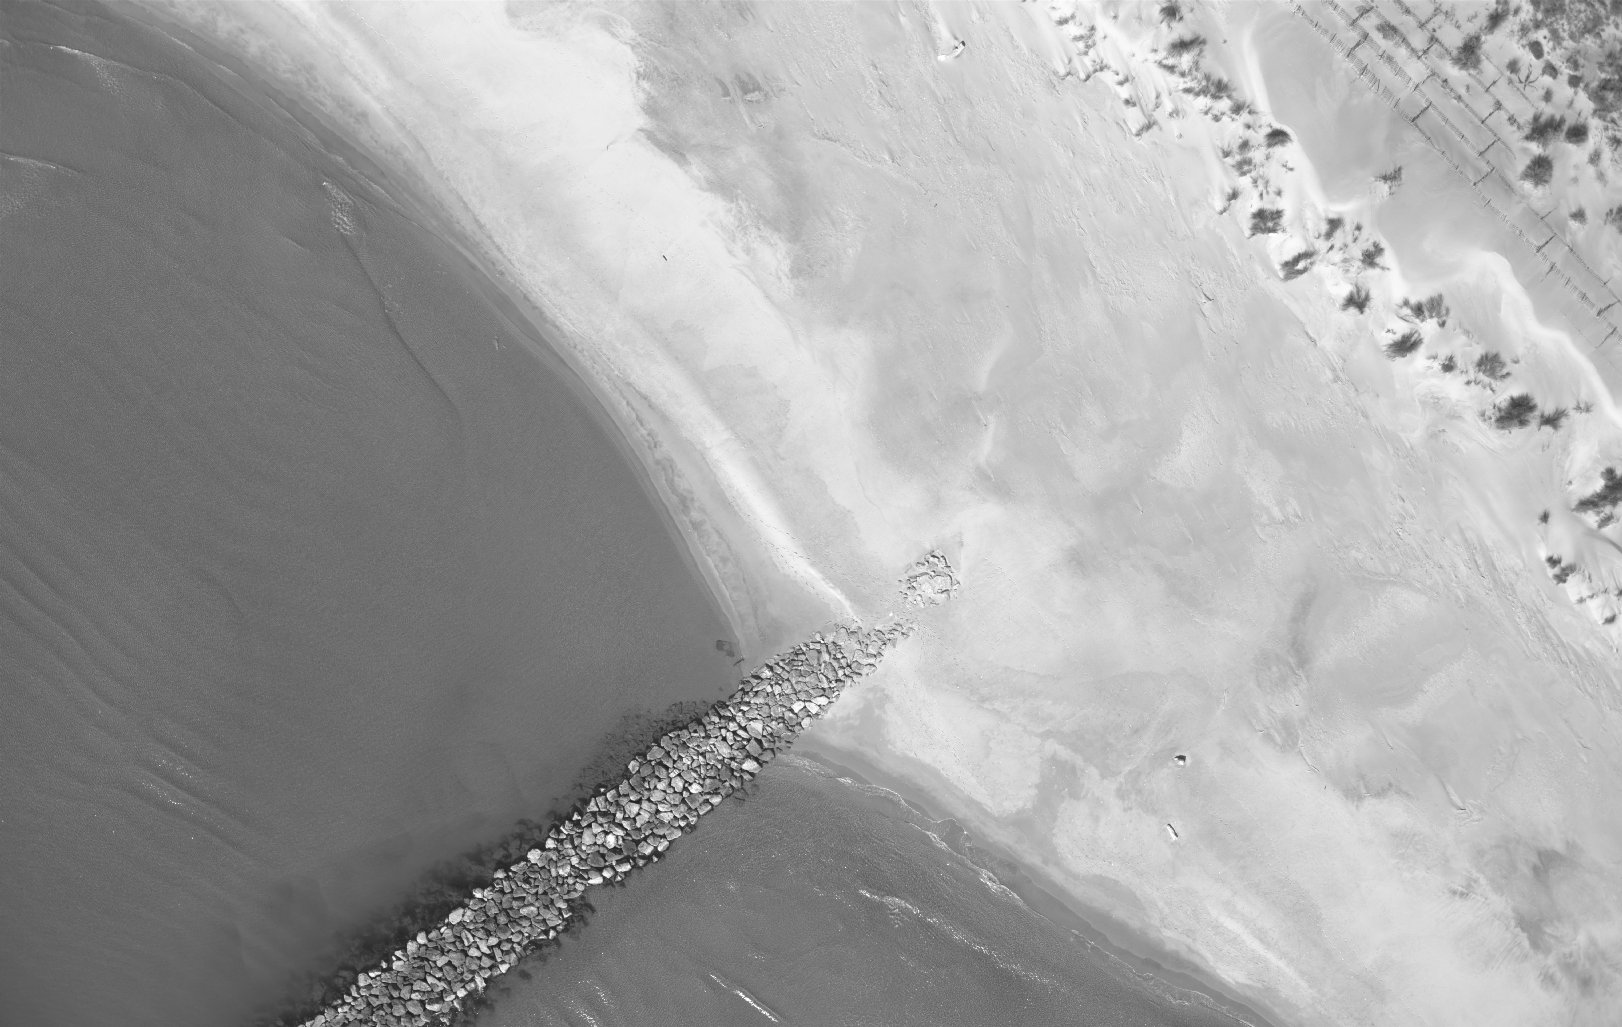
\includegraphics[width=0.95\textwidth]{FIGS/Tapioca-SFS/Im-STD.jpg}

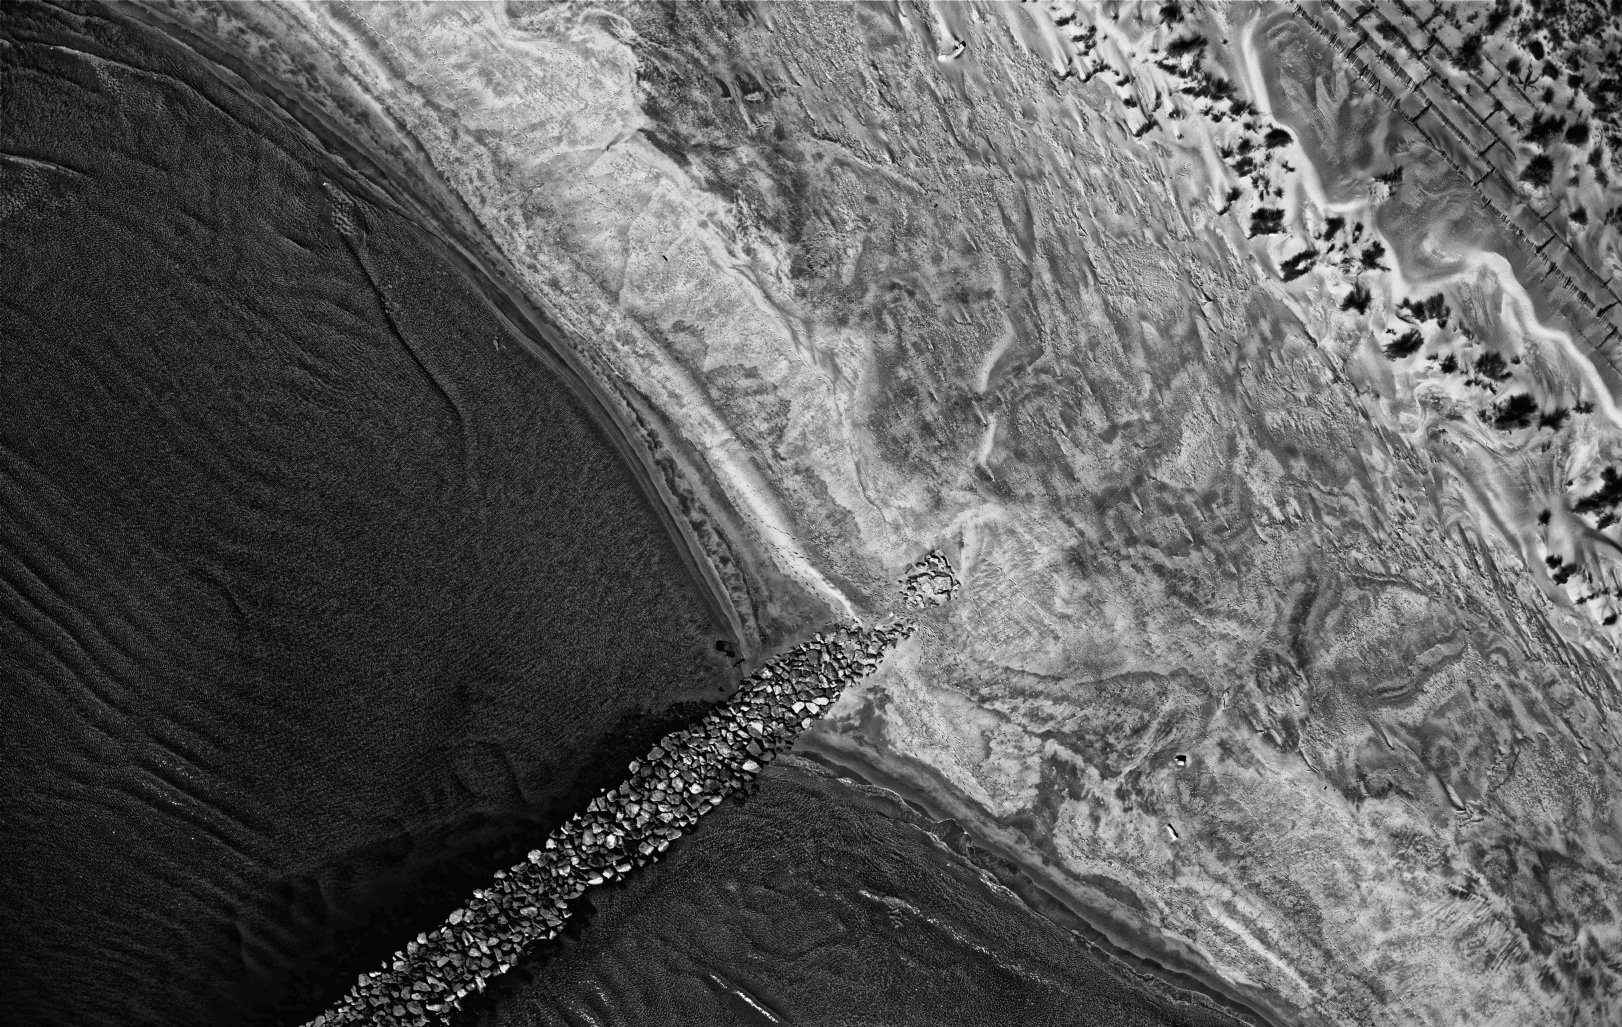
\includegraphics[width=0.95\textwidth]{FIGS/Tapioca-SFS/Im-SFS.jpg}
\end{center}
\caption{Global images before and after enhancement}
\label{FIG:SF:Img}
\end{figure}

%=======================================================================================================

\newpage

\section{Tie point reduction in {\tt RedTieP}}


This command can be used to reduce the number of tie points generated by \textit{Tapioca}. Currently it requires to format the \textit{Homol} folder into the Martini format, so before executing \textit{RedTieP} one has to execute the tool \textit{NO\_AllOri2Im} (obviously, after running \textit{Tapioca} to compute the tie-points):

The command {\tt RedTieP} keeps the tie-points that are present in a higher number of images and that guarantee a good distribution in the pixel-space of the images. 

\begin{verbatim}
 mm3d RedTieP
*****************************
*  Help for Elise Arg main  *
*****************************
Mandatory unnamed args : 
  * string :: {Pattern of images}
Named args : 
  * [Name=NumPointsX] INT :: {Target number of tie points between 2 images in x axis of 
                              image space, def=4}
  * [Name=NumPointsY] INT :: {Target number of tie points between 2 images in y axis of 
                              image space, def=4}
  * [Name=SubcommandIndex] INT :: {Internal use}
  * [Name=ExpSubCom] bool :: {Export the subcommands instead of executing them, def=false}
  * [Name=ExpTxt] bool :: {Export homol point in Ascii, def=false}
  * [Name=SortByNum] bool :: {Sort images by number of tie points, determining the order 
                              in which the subcommands are executed, def=0 
                              (sort by file name)}
  * [Name=Desc] bool :: {Use descending order in the sorting of images, def=0 (ascending)}
\end{verbatim}

The main options are :

\begin{enumerate}
\item The first option is mandatory and it is the patter to be used to select the images.

\item {\tt NumPointsX} and {\tt NumPointsY} represent the target number of tie-points between an image pair (specified as \textit{numY}, i.e. \textit{numPointsTarget=numX*numY}).
   
\item {\tt SortByNum} to select if the sorting by file name or by number of tie-points (default is to sort by file name). This sorting has effect on the order in the processing workflow, the first image in the sorted list is the first one that has its tie-points reduced.

\item {\tt Desc} to indicate if use ascending or descending order when sorting the images to decide (default is ascending).

\item {\tt ExpTxt} is a boolean indicating if reduced tie-point are dumped in binary or ASCII format (default is binary).

\item \textit{ExpSubCom} is used to export the commands to perform the tie-point reduction pipeline without actually executing it. This is used to execute the pipeline with an external parallelization tool (see section below)
\end{enumerate}


\subsection{Algorithm description}

\begin{itemize}
\item Select the images from the pattern defined by the user. 

\item Sort the images. By default by file name in ascending order (user can choose to sort by number of tie-points, and/or to use descending order). 

\item Execute a set of tasks, one for each image. Each task executes various steps:
   \begin{itemize}
   
   \item Define a master image, the image driving the tie-point reduction in this task.
   
   \item Find the related images. The related images are images that share tie-points with the master image. 
   
   \item Load the tie-points shared between the master image and each of the related images. If a related image was a master image in a earlier executed task the algorithm uses the list of tie-points produced in that task (instead of the original list of tie-points as provided by Tapioca).

   \item Perform the topological merging of tie-points into multi-tie-points. A multi-tie-point stores in how many images a related tie-point is present (multiplicity) and its positions in those images. 
   
   \item For all the images including the master and the related images: 
      \begin{itemize}
      \item Create a grid that divides the image pixel-space. 
      
      \item Fill in the grid with the loaded multi-tie-points.
      \end{itemize}      
      
   \item For each cell of the master image grid:
      \begin{itemize}
       \item Sort the multi-tie-points according to multiplicity.
       \item Attempt to remove all the multi-tie-points in the grid cell except the one with higher multiplicity. A multi-tie-point can be deleted if it meets the following conditions:
          \begin{itemize}
          \item Condition 1: It is not present in a related image that was master in an earlier executed task.
          \item For each related image where the multi-tie-point has a tie-point: (Condition 2) there is at least another tie-point in the current master grid cell that is also shared with the related image, and (Condition 3) there is at least another tie-point in the grid cell of the related image. 
          \end{itemize}
      \end{itemize}
   \item Store the tie-points which have not been marked as deleteable.
   \end{itemize}
\end{itemize}

\subsection{Parallelization}

The \textit{RedTieP} executes the sets of tasks that perform the tie-point reduction using a single process and in sequential order. However, these tasks could be parallelized if the parallelization schema guarantees that there are never two tasks accessing the same set of tie-points (i.e. accessing the same files). Each tasks has mutual exclusion with some other tasks. In order to parallelize them we use a workflow execution engine called Noodles (https://github.com/NLeSC/noodles). A script that uses Noodles can be found in \textit{scripts/noodles\_exe\_pararallel.py}.

In order to run \textit{RedTieP} and parallelize it with Noodles use:
\begin{verbatim}
 mm3d RedTieP  {Pattern of images} ExpSubCom=1 
 python {MicMac path}/scripts/noodles_exe_pararallel.py -j {num. threads} subcommands.json
\end{verbatim}

To install Noodles Python 3.5 is required. We recommend downloading and installing Anaconda (https://www.continuum.io/). Then set an environment with Python 3.5, activate it and download and install Noodles:
\begin{verbatim}
git clone https://github.com/NLeSC/noodles.git
cd noodles
git checkout devel
pip install .
\end{verbatim}


